%!TEX root = forallxcam.tex
\part{Túlkanir}
\label{ch.semantics}

\chapter{Umtak}\label{s:Interpretations} %umtak er extension, en hvað er þá `extensionality'

Öll setningatengin í setningarökfræði eru, eins og við munum, sannföll (sjá \S\ref{s:TruthFunctionality}). Það þýðir að sanngildi setninganna ákvarðast eingöngu af sanngildum hlutasetninganna sem setningin samanstendur af. Það hefur í för með sér að þegar við þýðum setningar yfir á táknmál setningarökfræði, þá erum við í raun að tilgreina sanngildi setninganna. Þetta getum við gert með beinum hætti, með því einfaldlega að segja að tiltekin setning, til dæmis, $P$ eigi að vera sönn. Við gerum þetta meðal annars þegar við vinnum með sanntöflur. Þá úthlutum við tilteknum sanngildum fyrir hverja grunnsetningu í tiltekinni setningu.

En við getum líka tilgreint sanngildið \emph{óbeint}. Til dæmis þegar við tiltökum einhvern þýðingarlykil fyrir grunnsetningarnar sem koma fyrir í þeim setningum sem við erum að þýða. Hér er dæmi:
	\begin{ekey}
		\item[P] Sívali turn er í Kaupmannahöfn
	\end{ekey}
Hér erum við í raun ekki að ákveða að \emph{P} eigi að hafa \emph{merkinguna} „Sívali turn er í Kaupmannahöfn“, heldur frekar að \emph{P} eigi að hafa sama sanngildi og setningin „Sívali turn er í Kaupmannahöfn“. Þetta er í raun það sama og að hafa eftirfarandi línu í þýðingarlyklinum:
	\begin{ebullet}
		\item setningin `$P$' er sönn eff Sívali turn er í Kaupmannahöfn
	\end{ebullet}
Það er því ljóst að setningarökfræðin ræður ekki við blæbrigði í merkingu og einblínir eingöngu á sanngildi.

\section{Þýðing yfir á mál umsagnarökfræði}
Svipuðu máli gegnir um umsagnarökfræðina, en þó ekki alveg. Hún einblínir nefnilega ekki eingöngu á sanngildin, því hún gerir okkur kleift að brjóta setningar upp í einnefni, umsagnir og magnara. Á máli umsagnarökfræði getum því líka talað um hvað er \emph{satt um} tiltekinn hlut---eða suma eða alla hluti. En það er allt og sumt.

Við sjáum þetta kannski betur með að skoða eftirfarandi þýðingarlykil:
	\begin{ekey}
		\item[C] \gap{1} er rektor Háskóla Íslands þegar þessi bók er skrifuð
	\end{ekey} 
Þetta þýðir ekki að \emph{merking} íslensku umsagnarinnar hafi nú færst yfir á umsögnina í umsagnarökfræði. Við erum einfaldlega að ákveða að:
	\begin{ebullet}
		\item `$C$' skal vera satt um nákvæmlega þá hluti í yfirgripinu sem eru rektorar Háskóla Íslands þegar þessi bók er skrifuð, hvaða hlutir það svo sem eru.
	\end{ebullet}
Þetta væri óbein leið til tilgreina hvaða hluti þessi umsögn á að vera sönn um. En við gætum líka tilgreint það beint. Við gætum til að mynda sagt að umsögnin „C“ eigi að vera sönn um Jón Atla Benediktsson og engan annan en Jón Atla. Það vill svo til að í þessu tilfelli kemur þetta á sama stað niður, enda er Jón Atli eini rektor háskólans þegar þessi bók er skrifuð. En það er greinilegt að umsagnirnar „\blank\ er rektor Háskóla Íslands þegar þessi bók er skrifuð“ og „\blank\ er Jón Atli Benediktsson“ hafa greinilega ekki sömu merkingu!
	
Umsagnarökfræði er því sama marki brennd og setningarökfræðin, nefnilega að hún ræður ekki við öll blæbrigði merkingar. Þegar við tilgreinum nöfn og umsagnir umsagnarökfræðinnar þá erum við bara ákvarða hvað umsagnirnar eru sannar um. Stundum er sagt að umsagnarökfræðin sé \define{umtaksmál}. Við munum segja aðeins meira um þetta í næsta hluta.

\section{Nokkur orð um umtök}

Eins og áður segir, þá getum við tilgreint með beinum hætti hvaða hluti umsagnirnar okkar eiga að vera sannar um. Við gætum til dæmið ákveðið að „H“ eigi að vera satt---og aðeins satt um---eftirfarandi hluti:
	\begin{center}
		Katrín Jakobsdóttir\\
		töluna $\pi$\\
		allar harmóníkur sem nokkurn tíma hafa verið framleiddar
	\end{center}
Með þetta í huga, þá getum við bætt eftirfarandi við þýðingarlykilinn okkar:	
	\begin{ekey}
		\item[b] Bjarni Benediktsson
		\item[k] Katrín Jakobsdóttir
		\item[p] talan $\pi$
	\end{ekey}
Samkvæmt þessum þýðingarlykli eru setningarnar \emph{Hk} og \emph{Hp} báðar sannar, en \emph{Hb} ósönn, þar eð Bjarni Benediktsson er ekki Katrín Jakobsdóttir, harmóníka eða talan $\pi$. 
	
Að tilgreina hvaða hluti umsögn er sönn um með þessum hætti er stundum kallað að ákvarða \emph{umtak} umsagnarinnar---en með því er einfaldlega átt við þá hluti sem hún er sönn um. Umtak er í raun mengi allra þeirra hluta sem umsögnin er sönn um og þegar við segjum að tiltekið mál sé umtaksmál, þá eigum við við að sanngildi setningar á borð við \emph{Hk} ákvarðist eingöngu af því hvort hluturinn \emph{k} sé stak í menginu \emph{H}. Það er vert að veita því athygli að umtak umsagnar þarf ekki að samanstanda af hlutum sem eiga eitthvað ákveðið sameiginlegt. Frá sjónarhóli rökfræðinnar skiptir það engu.

\section{Margsæta umsagnir}
Þetta er tiltölulega einfalt þegar kemur að einsæta umsögnum. En þegar við bætum tvísæta umsögnum við, þá vandast málið. Tökum eftirfarandi þýðingarlykil sem dæmi:
	\begin{ekey}
		\item[E] \gap{1} elskar \gap{2}
	\end{ekey}
Í ljósi þess sem við sögðum að ofan, þá ætti að skilja þetta einhvern veginn svona:\footnote{Takið eftir því að „x“ og „y“ eru hérna tákn í framsetningarmálin, ekki tákn á máli umsagnarrökfræði.}
	\begin{earg}
		\item[\textbullet] `$E$' skal vera satt um \emph{x} og \emph{y} (í þessari röð) eff \emph{x} elskar \emph{y}. 
	\end{earg}
Það er mikilvægt að taka það fram að þetta beri að hafa í réttri röð, því eins og við vitum, þá er ást ekki alltaf endurgoldin.	

Hér höfum við tilgreint umtak umsagnarinnar með óbeinum hætti. En hvernig myndum við gera það beint? Ef við myndum bara tiltaka hvaða hlutir féllu undir „\emph{L}“, rétt eins og við gerðum fyrir einsæta umsagnir, þá myndum við ekki vita hver elskar hvern og hver er elskaður af hverjum. Við þurfum einhverja leið til að tilgreina í hvaða röð við viljum hafa hlutina.

Í þeim tilgangi getum við einfaldlega ákveðið að tvísæta umsagnir séu sannar um \emph{pör} af hlutum þar sem röðin er tekin fram. Við gætum til dæmis tiltekið að umsögnin „\emph{B}“ eigi að vera sönn um eftirfarandi pör og aðeins eftirfarandi pör:
	\begin{center}
		\ntuple{Lenín, Marx}\\
		\ntuple{Heidegger, Sartre}\\
		\ntuple{Sartre, Heidegger}
	\end{center}
Hér eiga oddklofarnir að sýna okkur í hvaða röð pörin eru. Segjum nú að við bætum eftirfarandi við þýðingarlykilinn:
	\begin{ekey}
		\item[l] Lenín
		\item[m] Marx
		\item[h] Heidegger
		\item[s] Sartre
	\end{ekey}
Þá sjáum við að setningin \emph{Blm} er sönn, enda er \ntuple{Lenín, Marx} á listanum okkar. \emph{Bml} er hins vegar ósönn, þar eð \ntuple{Marx, Lenín} er það ekki. Á hinn bóginn eru \emph{Bhs} og \emph{Bsh} báðar sannar því \ntuple{Heidegger, Sartre} og \ntuple{Sartre, Heidegger} eru báðar á listanum.

Til að gera þessar hugmyndir um umtak nákvæmar og fullkomlega skýrar þyrftum við að notast við dálítið af \emph{mengjafræði}. Hún hefur þau tæki og tól sem við þörfnumst til að gera sæmilega grein fyrir umtaki, röðuðum pörum (oftar kölluð „raðaðar tvenndir“ á íslensku), og svo framvegis. En mengjafræði er því miður ekki viðfangsefni þessarar bókar, svo við munum láta hér staðar numið í þeirri von að þetta sé þó þokkalega skýrt.

\section{Merkingarfræði samsemdar}
Samsemd er óvenjuleg umsögn í umsagnarökfræði og eins og áður hefur komið fram, þá ritum við hana á annan hátt en aðrar tvísæta umsagnir: í stað „Ixy“, til dæmis, þá ritum við $x=y$. En mikilvægara er þó að merking hennar er alltaf sú sama, nefnilega að einnefnin sem eru sitthvorum megin við samsemdarmerkið séu sami hluturinn. 

Tökum nú eftir því að ef tvö nöfn vísa til sama hlutar, þá breytir það ekki sanngildi setningar að skipta út einu nafni fyrir annað í hvaða setningu sem er. Til dæmis, ef „a“ og „b“ vísa til sama hlutar, þá eru eftirfarandi setningar allar sannar: \label{model.nonidentity}
	\begin{align*}
	 	Aa &\eiff Ab \\
	 	Ba &\eiff Bb\\
		Raa &\eiff Rbb\\
		Raa & \eiff Rab\\
		Rca &\eiff Rcb\\
		\forall x Rxa &\eiff \forall x Rxb
	\end{align*}
Sumir heimspekingar hafa trúað hinu gagnstæða, nefnilega að þegar allar sömu setningar (þó ekki þær sem innihalda „=“) eru sannar um \textbf{a} og \emph{b}, þá eru \emph{a} og \emph{b} sami hluturinn. Þetta er mjög umdeild heimspekileg skoðun (og er oft kölluð \emph{lögmálið um samsemd óaðgreinanlegra hluta}) og fellst umsagnarökfræðin ekki á hana. Samkvæmt henni er það vel mögulegt að nákvæmlega sömu umsagnir eigi við um tvo aðskilda hluti.

Tökum eftirfarandi þýðingarlykil sem dæmi:
	\begin{ebullet}
		\item[\text{yfirgrip}:] Finnur Dellsén, Ásgeir Berg Matthíasson
		\item[$f$:] Finnur Dellsén
		\item[$a$:] Ásgeir Berg Matthíasson
		\item Sama hvaða umsögn við látum okkur detta í hug, sú umsögn er ekki sönn um \emph{neitt}
			\end{ebullet}
Segjum nú sem dæmi að \emph{A} sé einsæta umsögn. Þá er \emph{Aa} ósatt, sem og \emph{Af}. En $Aa \eiff Af$ er satt. Eins væri \emph{Raa} ósatt, ef \emph{R} er tvísæt umsögn, rétt eins og $Raf$. En $Raa \eiff Raf$ væri aftur á móti sönn. Samkvæmt þessum þýðingarlykli eru því allar grunnsetningar sem ekki innihalda „=“ ósannar og allar jafngildissetningar sem tengja saman slíkar setningar sannar. En þó eru Ásgeir og Finnur ekki sami maðurinn!		
			
\section{Túlkanir}
Við skilgreindum \emph{sanngildadreifingu} í setningarökfræði sem tiltekna úthlutun sanngilda á allar grunnsetningar í setningu. Í umsagnarökfræði köllum við samsvarandi fyrirbæri \define{túlkun}. Til að setja fram túlkun á einhverjum tilteknum setningum þarf að gera þrennt:
	\begin{ebullet}	
		\item að tilgreina yfirgrip
		\item fyrir hvert nafn sem kemur fyrir í setningunum þarf að tilgreina nákvæmlega einn hlut í yfirgripinu
		\item fyrir hverja umsögn sem kemur fyrir í setningunum (fyrir utan $=$) þarf að tilgreina umtak þeirra---hvaða hluti þær eiga að vera sannar um. (Við þurfum ekki að gera þetta fyrir $=$ sem alltaf hefur sömu túlkun.)
	\end{ebullet}
Þýðingarlyklarnir sem við kynntum til sögunnar í \ref{ch.FOL} eru hentug leið til að setja fram túlkanir. Við munum halda áfram að nota þá í þessum kafla.

En það getur líka verið þægilegt að setja túlkun fram \emph{myndrænt}. Segjum til dæmis að við viljum skoða eina tvísæta umsögn, $R$. Við gætum tilgreint umtak hennar með því að teikna mynd þar sem ör er dregin á milli tveggja hluta og sagt að $R$ eigi við \emph{x} og \emph{ y} ef og aðeins ef það er ör frá \emph{x} til \emph{y} á myndinni (og athugið að ör frá \emph{x} til \emph{y} er ekki það sama og ör frá \emph{y} til \emph{x}. Þannig getum við tilgreint \emph{röð} hlutanna.) Hér er dæmi:
\begin{center}
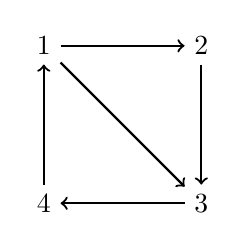
\begin{tikzpicture}
\node (atom1) at (0,2) {1};
\node (atom2) at (2,2) {2};
\node (atom3) at (2,0) {3};
\node (atom4) at (0,0) {4};
\draw[->, thick] (atom1)--(atom2);
\draw[->, thick] (atom2)--(atom3);
\draw[->, thick] (atom3)--(atom4);
\draw[->, thick] (atom4)--(atom1);
\draw[->, thick] (atom1) -- (atom3);
\end{tikzpicture}
\end{center}
Eftirfarandi mynd gæti lýst túlkun þar sem yfirgripið eru fyrstu fjórar heiltölurnar og \emph{R} er satt um (og aðeins satt um) eftirfarandi:
	\begin{center}
		\ntuple{1, 2}, 
		\ntuple{2, 3}, 
		\ntuple{3, 4}, 
		\ntuple{4, 1}, 
		\ntuple{1, 3}
	\end{center}
Við gætum líka tekið eftirfarandi mynd:

\begin{center}
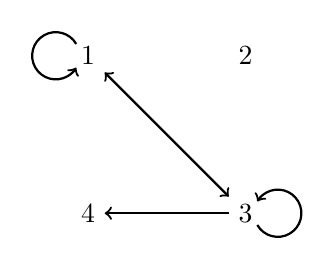
\begin{tikzpicture}
\node (atom1) at (0,2) {1};
\node (atom2) at (2,2) {2};
\node (atom3) at (2,0) {3};
\node (atom4) at (0,0) {4};
\draw[->, thick] (atom3)--(atom4);
\draw[->, thick] (atom1)+(-0.15,0.15) arc (-330:-30:.3); 
\draw[->, thick] (atom3)+(0.15,-0.15) arc (-150:150:.3); 
\draw[<->, thick] (atom1) -- (atom3);
\end{tikzpicture}
\end{center}
sem dæmi um túlkun með sama yfirgrip, þar sem umtak $R$ er:
	\begin{center}
		\ntuple{1, 3}, 
		\ntuple{3, 1}, 
		\ntuple{3, 4}, 
		\ntuple{1, 1},
		\ntuple{3, 3}
	\end{center}
Ef við viljum, þá getum við líka teiknað flóknari myndir. Við gætum til að mynda bætt nöfnum inn sem merkimiða á tiltekna hluti. Við gætum líka táknað umtak einsæta umsagnar með því að draga hring utan um þá hluti sem hún á að vera sönn um (og aðeins þá). Það sem mestu skiptir er að túlkunin tilgreini yfirgrip og umtak setninganna (og til hvaða hluta nöfnin eiga að vísa, ef við notum þau).

\chapter{Sannleikur í umsagnarökfræði}\label{s:TruthFOL}
Túlkanir segja okkur um hvaða hluti í yfirgripinu umsagnir eru sannar um og til hvaða hluta nöfnin sem við notum vísa. Þær segja okkur með öðrum orðum hvaða grunnsetningar eru sannar og hverjar ekki. Það sem okkur vantar þá er að geta sagt um \emph{allar} setningar í umsagnarökfræði hvort þær séu sannar eða ósannar---að einhverri túlkun gefinni.

Við lærðum í kafla \S\ref{s:FOLSentences} að það eru þrjár tegundir af setningum í umsagnarökfræði:
	\begin{ebullet}
		\item grunnsetningar
		\item setningar sem hafa setningatengi sem aðalvirkja
		\item setningar sem hafa magnara sem aðalvirkja
	\end{ebullet}
Við þurfum því að skilgreina hvað sannleikur í umsagnarökfræði er fyrir allar þessar þrjár gerðir setninga.	

Slík skilgreining verður, eðli málsins samkvæmt, að vera fullkomlega almenn. En í því skyni að gera umfjöllunina skýrari, þá mun ég á köflum notast við eftirfarandi túlkun:
	\begin{ekey}
		\item[\text{yfirgrip}] fólk fætt fyrir árið 2000\textsc{ce}
		\item[a] Aristóteles
		\item[d] Donald Trump
		\item[V] \gap{1} er vitur
		\item[R] \gap{1} fæddist á undan \gap{2}
	\end{ekey}
Þessi túlkun verður notuð sem dæmi þegar við á.	
\section{Grunnsetningar}
Sanngildi grunnsetninga er tiltölulega einfalt mál. Setningin \emph{Va} ætti að vera sönn ef og aðeins ef umsögnin \emph{V} er sönn um \emph{a}. Ef við miðum við þá túlkun sem gefin var hér að ofan, þá er þetta satt ef og aðeins ef Aristóteles er vitur. Aristóteles er vitur, svo setningin er sönn.\footnote{Það er að segja, ef við hunsum tíð sagnarinnar. Það eru til önnur rökfræðikerfi sem reyna að fanga tíðir sagna, en klassísk umsagnarökfræði er ekki ein af þeim.} Á sama hátt gætum við sýnt að setningin \emph{Vd} sé ósönn samkvæmt þessari túlkun.

Hvað með tvísæta umsagnirnar? \emph{Rad} er sönn ef og aðeins ef sá hlutur í yfirgripinu sem \emph{a} nefnir er fæddur á undan þeim hlut sem \emph{d} nefnir. Aristóteles fæddist vissulega á undan Donald Trump, svo \emph{Rad} er sönn. \emph{Raa} er ósönn, því Aristóteles fæddist ekki á undan Aristótelesi.

Það liggur því beint við að segja:
	\factoidbox{
		Ef \meta{R} er $n$-sæta umsögn og $\meta{a}_1, \meta{a}_{2}, \ldots, \meta{a}_{n}$ eru nöfn, þá er setningin $\meta{R}\meta{a}_{1}\meta{a}_{2}\ldots\meta{a}_{n}$ sönn samkvæmt tiltekinni túlkun, ef og aðeins ef R er sönn um þá hluti sem $\meta{a}_{1}, \meta{a}_{2}, \ldots, \meta{a}_{n}$ (í þessari röð) nefna samkvæmt þeirri sömu túlkun.
		}
Við megum þó ekki gleyma að það er til ein önnur gerð grunnsetninga, nefnilega setningar sem innihalda samsemdarmerkið. Um þær segjum við:
	\factoidbox{
		Ef $\meta{a}$ og $\meta{b}$ eru nöfn, þá er setningin $\meta{a} = \meta{b}$ sönn samkvæmt ákveðinni túlkun ef og aðeins ef
		 \meta{a} og \meta{b} nefna sama hlut samkvæmt þeirri sömu túlkun.
	}
Ef við skoðum aftur túlkunina sem gefin var hér að ofan, þá er setningin $a = d$ ósönn, þar eð \emph{a} nefnir Aristóteles en \emph{d} nefnir Donald Trump---og Aristóteles og Trump eru ekki sami hluturinn. Á hinn bóginn er $a = a$ sönn, þar sem Aristóteles er sami hluturinn og Aristóteles!

\section{Setningatengi}

Við lærðum í \S\ref{s:FOLSentences} að setningar í umsagnarökfræði eru smíðaðar úr einfaldari setningum með sömu setningatengjum og við kynntumst í setningarökfræðinni. Reglurnar sem ákvarða sannleika fyrir setningar í umsagnarökfræði sem hafa setningatengi sem aðalvirkja (en ekki magnara) eru því nákvæmlega þær sömu og fyrir setningar í setningarökfræði. Hér eru þær:
	\factoidbox{
		$\meta{A} \eand \meta{B}$ er sönn skv.\ tiltekinni túlkun \textbf{eff}\\ $\meta{A}$ og $\meta{B}$ eru báðar sannar skv.\ sömu túlkun \\ \\		
		$\meta{A} \eor \meta{B}$ er sönn skv.\ tiltekinni túlkun \textbf{eff}\\ annað hvort $\meta{A}$ er sönn eða $\meta{B}$ er sönn skv.\ sömu túlkun \\ \\
		$\enot \meta{A}$ er sönn skv.\ tiltekinni túlkun \textbf{eff}\\$\meta{A}$ er ósönn skv.\ sömu túlkun \\ \\
		$\meta{A} \eif \meta{B}$ er sönn skv.\ tiltekinni túlkun \textbf{eff}\\ annað hvort $\meta{A}$ er ósönn eða $\meta{B}$ er sönn skv.\ sömu túlkun \\ \\
		$\meta{A} \eiff \meta{B}$ er sönn skv.\ tiltekinni túlkun \textbf{eff}\\$\meta{A}$ hefur sama sanngildi og $\meta{B}$ skv.\ sömu túlkun
	}
En hvernig má vera að þetta séu sömu reglur? Skilgreindum við ekki sannleika í setningarökfræði með sanntöflum? Jú, en þrátt fyrir að vera á öðru formi, þá segja þessar reglur það sama. Við gætum meira að segja litið á þær sem \emph{lýsingu} á sanntöflunum okkar. Til dæmis, ef við myndum skoða sanntöfluna fyrir og-tengið, þá sæjum við að $\meta{A} \eand \meta{B}$ er bara sönn á þeirri línu þar sem \meta{A} er sönn og \meta{B} er sönn, en ósönn annars staðar---rétt eins og reglan fyrir og-tengið segir hér. Sama gildir um hinar reglurnar.

Hér eru nokkur dæmi um setningar til glöggvunar:
	
	\begin{earg}
		\item[\textbullet] $a = a \eand Va$ er sönn
		\item[\textbullet] $Rad \eand Vd$ er ósönn, því jafnvel þó $Rad$ sé sönn, þá er $Vd$ ósönn
		\item[\textbullet] $a = d \eor Va$ er sönn
		\item[\textbullet] $a \neq d$ er sönn
		\item[\textbullet] $Va \eand \enot( a= d \eand Rad)$ er sönn, því $Va$ er sönn og $a = d$ er ósönn
	\end{earg}

\section{Setningar með magnara sem aðalvirkja}\label{s:MainLogicalOperatorQuantifier}

Það sem greinir umsagnarökfræðina frá setningarökfræðinni eru þó auðvitað \emph{magnararnir} og það vill svo til að það er ekki alveg jafn auðvelt að skilgreina sannleika fyrir þá og maður myndi kannski halda. Hér er ein hugmynd: Við viljum segja að $\forall x Fx$ sé sönn eff $Fx$ er sönn um allt í yfirgripinu. Af hverju ekki bara að láta túlkunina sjá um þetta, enda segir hún til um það hvort $F$ sé satt um allt í yfirgripinu eða ekki?

En því miður er þessi lausn ekki nógu almenn. Munum að setningar í umsagnarökfræði eru byggðar upp í skrefum, úr öðrum setningum, og við viljum geta sagt um \emph{allar} setningar hvenær þær eru sannar og hvenær ekki. Hvað þá um $\forall x \exists y Lxy$ til að mynda? Þessi setning ætti að vera sönn ef og aðeins ef $\exists y Lxy$ er sönn um allt í yfirgripinu. En túlkunin getur ekki sagt okkur neitt um það. Við viljum því að það \emph{leiði af} túlkuninni og merkingu magnaranna að $\exists y Lxy$ sé sönn.

Hér er því önnur hugmynd. Við gætum reynt að segja að $\forall x \exists y Lxy$ sé sönn eff $\exists y L\meta{a}y$ er sönn fyrir \emph{öll} nöfn \meta{a} sem við höfum tiltekið. Á svipaðan hátt gætum við sagt að $\exists y L\meta{a}y$ sé sönn eff $L\meta{a}\meta{b}$ er sönn fyrir \emph{eitthvað} nafn \meta{b} í túlkuninni.xw

Þetta væri vissulega skref í rétta átt, en því miður dugir það ekki til. Til að sjá það, skoðum aftur túlkunina sem við tilgreindum í upphafi þessa kafla. Þar höfum við bara tvö nöfn, $a$ og $d$. En yfirgripið inniheldur allt fólk fætt fyrir árið 2000---sem eru að sjálfsögðu mun, mun fleiri! Við höfum hvorki vilja né getu til að nefna allt þetta fólk í yfirgripinu en viljum samt geta sagt eitthvað um það með mögnurum.

Hér er því þriðja hugmyndin: Það er vissulega rétt að við höfum ekki nefnt allt í yfirgripinu í túlkuninni, en \emph{fræðilega} séð væri það mögulegt. Það skiptir jú ekki máli hversu mörg nöfn við höfum í túlkuninni, við gætum alltaf bætt einu við í viðbót---víkkað túlkunina út. Skoðum þessa hugmynd aðeins betur áður en við gefum almenna skilgreiningu.

Í túlkuninni sem við höfum notað sem dæmi hingað til ætti setningin $\exists x Rdx$ að vera sönn. Það eru jú margir í yfirgripinu sem fæddust á eftir Donald Trump. Til dæmis Björk Guðmundsdóttir. Ef við myndum tímabundið víkka út túlkunina okkar og bæta nafninu $b$ sem vísaði til Bjarkar við túlkunina, þá myndi setningin $Rdb$ nú vera sönn (samkvæmt þessari nýju, útvíkkuðu túlkun). Það sýnir að $\exists x Rdx$ hlýtur að vera satt samkvæmt upprunalegu túlkuninni (munið: við bættum Björk ekki við yfirgripið, enda var hún þar þá þegar, heldur bættum við við \emph{nafni} sem vísaði til hennar).

Setningin $\exists x (Vx \eand Rxa)$ ætti líka að vera sönn. Sókrates var jú vitur og fæddist á undan Aristótelesi. Ef við bættum nýju nafni, $c$, við túlkunina og létum það vísa til Sókratesar, þá væri setningin $Vc \eand Rca$ greinilega sönn samkvæmt þessari útvíkkuðu túlkun. Rétt eins og áður, þá myndi það sýna að $\exists x (Vx \eand Rxa)$ hlýtur að vera sönn samkvæmt upprunalegu túlkuninni.

Skoðum eitt dæmi til viðbótar. Samkvæmt túlkuninni ætti $\forall x \exists y Rxy$ að vera ósönn setning. Hún segir að allir í yfirgripinu séu þannig að það sé einhver sem er fæddur á eftir þeim. Ef við prófuðum því að taka síðustu manneskjuna sem fæddist árið 1999 og úthluta henni nafni, segjum $l$, þá gætum við ekki fundið neinn annan, sem við getum til dæmis kallað $m$, í yfirgripinu sem er þannig að $Rlm$. Það skiptir engu máli hver í yfirgripinu fengi úthlutað nafninu $m$, þessi setning væri alltaf ósönn. Það sýnir að $\exists y Rly$ er ósönn samkvæmt upprunalegu túlkuninni.

Með þessi dæmi í huga, þá getum við loks gefið almenna skilgreiningu á sannleika fyrir setningar í umsagnarökfræði sem hafa magnara sem aðalvirkja. Þessi skilgreining er því miður ekki sérlega falleg og við þurfum að kynna til sögunnar nokkur ný hugtök áður en við byrjum. 

Segjum að \meta{A} sé formúla sem inniheldur að minnsta kosti eitt tilvik af breytunni \meta{x} og að \meta{x} sé óbundin í \meta{A}. Við skrifum þá:
$$\meta{A}(\ldots \meta{x} \ldots \meta{x} \ldots)$$
Segjum líka að \meta{c} sé nafn. Þá munum við skrifa:
$$\meta{A}(\ldots \meta{c} \ldots \meta{c} \ldots)$$
fyrir þá formúlu sem fæst með að skipta \meta{x} í \meta{A} út fyrir \meta{c} alls staðar þar sem \meta{x} kemur fyrir. Við köllum þessa formúlu \define{innsetningartilvik} af $\forall \meta{x}\meta{A}$ og $\exists\meta{x}\meta{A}$. Við köllum \meta{c} \define{innsetningarnafn}. Innsetningartilvik er með öðrum orðum sú formúla sem fæst með að taka magnara framan af annarri formúlu og skipta þeirri breytu sem magnarinn batt út fyrir eitthvað nafn. Formúlan
	$$\exists x (Rex \eiff Fx)$$
er því innsetningartilvik af formúlunni
	$$\forall y \exists x (Ryx \eiff Fx)$$
með innsetningarnafnið $e$.

Með þennan rithátt að vopni getum við loksins skilgreint sannleika fyrir setningar sem hafa magnara sem aðalvirkja. Við getum sagt að setningin $\forall \meta{x}\meta{A}(\ldots \meta{x} \ldots \meta{x} \ldots)$ sé sönn ef og aðeins ef $\meta{A}(\ldots \meta{c} \ldots \meta{c}\ldots)$ er sönn sama hvaða hlut í yfirgripinu nafnið $\meta{c}$ nefnir. Eins getum við sagt að setningin $\exists \meta{x}\meta{A}$ sé sönn ef og aðeins ef það er hægt að finna hlut í yfirgripinu og gefa honum nafnið \meta{c} þannig að setningin $\meta{A}(\ldots \meta{c} \ldots \meta{c} \ldots)$ sé sönn.

Með örlítið nákvæmari og formlegri hætti segjum við:
	\factoidbox{
		$\forall \meta{x}\meta{A}(\ldots \meta{x}\ldots\meta{x}\ldots)$ er sönn samkvæmt tiltekinni túlkun \textbf{eff}\\$\meta{A}(\ldots \meta{c} \ldots \meta{c}\ldots)$ er sönn fyrir \emph{hvaða} aðra túlkun sem útvíkkar upprunalegu túlkunina þannig að einhverjum hlut í yfirgripinu er gefið nafnið \meta{c} (án þess þó að breyta upprunalegu túlkuninni á nokkurn hátt annan)\\ \\
		$\exists \meta{x}\meta{A}(\ldots \meta{x}\ldots\meta{x}\ldots)$ er sönn samkvæmt tiltekinni túlkun \textbf{iff}\\ 
		$\meta{A}(\ldots \meta{c}\ldots\meta{c}\ldots)$ fyrir \emph{einhverja} aðra túlkun sem útvíkkar upprunalegu túlkunina þannig að einhverjum hlut í yfirgripinu er gefið nafnið \meta{c} (án þess þó að breyta upprunalegu túlkuninni á nokkurn hátt annan)
	}
Það eina sem skilgreiningin í kassanum hér að ofan gerir er að skilgreina---kannski of---nákvæmlega þessa óformlegu hugmynd um útvíkkun sem kynnt var hér að ofan. Hún kann kannski að virðast helstu óskýr og tyrfin, en vonandi er hugmyndin þar að baki það ekki.

\practiceproblems
\problempart
\label{pr.TorF1}
Skoðið eftirfarandi túlkun (og hafið í huga að það er engin skylda að hafa nöfn yfir allt í yfirgripinu):
	\begin{ebullet}
		\item yfirgripið samanstendur af Önnu og Jóni
		\item `$A$' er einsæta umsögn og sönn um Jón og Önnu
		\item `$B$' er einsæta umsögn og bara sönn um Önnu
		\item `$N$' er einsæta umsögn og ekki sönn um neitt
		\item `$j$' vísar til Jóns
	\end{ebullet}
Segið til um hvort eftirfarandi setningar séu sannar eða ósannar samkvæmt þessari túlkun:
\begin{earg}
\item $Bj$
\item $Aj \eiff \enot Nj$
\item $Nj \eif (Aj \eor Bj)$
\item $\forall x Ax$
\item $\forall x \enot Bx$
\item $\exists x(Ax \eand Bx)$
\item $\exists x(Ax \eif Nx)$
\item $\forall x(Nx \eor \enot Nx)$
\item $\exists x Bx \eif \forall x Ax$
\end{earg}

\problempart
Skoðið eftirfarandi túlkun:	
	\begin{ebullet}
		\item Yfirgripið samanstendur af Kasper, Jesper og Jónatan
		\item `$G$' er einsæta umsögn og sönn um Kasper, Jesper og Jónatan
		\item `$H$' er einsæta umsögn og bara sönn um Kasper
		\item `$M$' er einsæta umsögn og bara sönn um Jesper og Jónatan
		\item `$k$' vísar til Kaspers
		\item `$j$' vísar Jespers
	\end{ebullet}
Segið til um hvort eftirfarandi setningar séu sannar eða ósannar samkvæmt þessari túlkun:
\begin{earg}
\item $Hk$
\item $Hj$
\item $Mk \eor Mj$
\item $Gk \eor \enot Gk$
\item $Mk \eif Gk$
\item $\exists x Hx$
\item $\forall x Hx$
\item $\exists x \enot Mx$
\item $\exists x(Hx \eand Gx)$
\item $\exists x(Mx \eand Gx)$
\item $\forall x(Hx \eor Mx)$
\item $\exists x Hx \eand \exists x Mx$
\item $\forall x(Hx \eiff \enot Mx)$
\item $\exists x Gx \eand \exists x \enot Gx$
\item $\forall x\exists y(Gx \eand Hy)$
\end{earg}

\problempart
\label{pr.TorF3}
Skoðið umfjöllunina um myndræna framsetningu á túlkunum hér að ofan í \S\ref{s:Interpretations} og skoðið eftirfarandi túlkun:	
\begin{center}
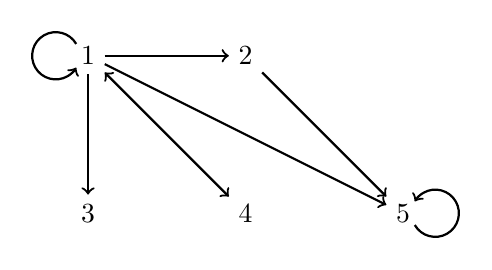
\begin{tikzpicture}
\node (atom1) at (0,2) {1};
\node (atom2) at (2,2) {2};
\node (atom4) at (0,0) {3};
\node (atom5) at (2,0) {4};
\node (atom6) at (4,0) {5};
\draw[->, thick] (atom1)+(-0.15,0.15) arc (-330:-30:.3); 
\draw[->, thick] (atom6)+(0.15,-0.15) arc (-150:150:.3); 
\draw[->, thick] (atom1) -- (atom2);
\draw[->, thick] (atom1) -- (atom4);
\draw[<->, thick] (atom1) -- (atom5);
\draw[->, thick] (atom1) -- (atom6);
\draw[->, thick] (atom2) -- (atom6);
\end{tikzpicture}
\end{center}
Segið til um hvort eftirfarandi setningar séu sannar eða ósannar samkvæmt þessari túlkun:
\begin{earg}
\item $\exists x Rxx$
\item $\forall x Rxx$
\item $\exists x \forall y Rxy$
\item $\exists x \forall y Ryx$
\item $\forall x \forall y \forall z ((Rxy \eand Ryz) \eif Rxz)$
\item $\forall x \forall y \forall z ((Rxy \eand Rxz) \eif Ryz)$
\item $\exists x \forall y \enot Rxy$
\item $\forall x(\exists y Rxy \eif \exists y Ryx)$
\item $\exists x \exists y (\enot x = y \eand Rxy \eand Ryx)$
\item $\exists x \forall y(Rxy \eiff x = y)$
\item $\exists x \forall y(Ryx \eiff x = y)$
\item $\exists x \exists y(\enot x = y \eand Rxy \eand \forall z(Rzx \eiff y = z))$
\end{earg}


\chapter{Merkingarfræðileg hugtök}
Að skilgreina sannleika í umsagnarökfræði var ansi snúið. En nú þegar við erum komin með skilgreininguna í hús getum við notað hana til að skilgreina önnur mikilvæg hugtök. Við höfum áður skilgreint sambærileg hugtök fyrir setningarökfræði í kafla \S\ref{s:semanticconcepts} en þau byggðu að sjálfsögðu á skilgreiningunni á sannleika fyrir setningarökfræði, sem byggðist á sanngildadreifingum, en ekki túlkunum. Þær eru í forgrunni hér. Að öðru leyti er ekkert nýtt á ferðinni.

\
\\Við notum táknið $\entails$ rétt eins og áður:
	$$\meta{A}_1, \meta{A}_2, \ldots, \meta{A}_n \entails\meta{C}$$
þýðir að það er ekki til nein túlkun sem gerir $\meta{A}_1, \meta{A}_2, \ldots, \meta{A}_n$  sanna og \meta{C} ósanna og við segjum að \meta{C} leiði rökfræðilega af $\meta{A}_1, \meta{A}_2, \ldots, \meta{A}_n$.

\
\\Ef $\meta{C}$ er sönn fyrir hvaða túlkun sem er, þá ritum við:
	$$\phantom{\meta{A}} \entails\meta{C}$$
Þá segjum við að $\meta{C}$ séu \define{röksannindi}. Röksannindi samsvarar klifun í setningarökfræði.

\
\\En á hinn bóginn, ef $\meta{A}$ er ósönn fyrir hvaða túlkun sem er, þá skrifum við:
$$\meta{A} \entails \phantom{\meta{C}}$$
Við köllum $\meta{A}$ þá \define{mótsögn}.

\
\\
Ef við viljum segja að það sé \emph{ekki} satt að $\meta{A}_1, \ldots, \meta{A}_n \entails \meta{C}$, þá strikum við yfir táknið fyrir rökfræðilega afleiðingu og segjum: 
$$\meta{A}_1, \meta{A}_2, \ldots, \meta{A}_n \nentails\meta{C}$$
Þetta þýðir að er til túlkun sem er þannig að setningarnar $\meta{A}_1,\ldots, \meta{A}_n$ eru allar sannar, en $\meta{C}$ er ósönn.
\
\\Tvær setningar í umsagnarökfræði \meta{A} og \meta{B} er \define{rökfræðilega jafngildar} eff þær eru sannar í nákvæmlega sömu túlkunum. Það er að segja, ef $\meta{A}\entails\meta{B}$ og $\meta{B}\entails\meta{A}$.

\
\\Eitthvert safn af setningum í umsagnarökfræði eru \define{rökfræðilega samkvæmar} ef og aðeins ef til er einhver túlkun þar sem þær eru allar sannar. Þær eru svo loks \define{rökfræðilega ósamkvæmar} eff engin slík túlkun er til.

\chapter{Að vinna með túlkanir}
\label{sec.UsingModels}

\section{Röksannindi og mótsagnir}
Gerum ráð fyrir að við viljum sýna að $\exists xAxx \eif Bd$ séu \emph{ekki} röksannindi. Í samræmi við skilgreininguna þurfum við þá að sýna að setningin sé ekki sönn fyrir allar túlkanir; það er að segja, að hún sé ósönn fyrir einhverja túlkun. Ef við getum því fundið eina einustu túlkun þar sem setningin er ósönn, þá höfum við sýnt að setningin sé ekki röksannindi.

Hvernig ættum við þá að bera okkur að? Við vitum að $\exists xAxx \eif Bd$ er ósönn, ef forliðurinn ($\exists x Axx$) er sannur og bakliðurinn ($Bd$) er ósannur. Við þurfum því að \emph{búa til} túlkun sem er þannig að þessi skilyrði eru uppfyllt. Við byrjum á því að tilgreina yfirgrip. Það er auðveldast að reyna að halda yfirgripinu eins litlu og mögulegt er, svo við bætum bara einum hlut við það. Segjum bara Dalvík.
	\begin{ekey}
		\item[\text{yfirgrip}] Dalvík
	\end{ekey}
Munum: Við erum að reyna að gera setninguna $Bd$ ósanna og við höfum bara einn hlut í yfirgripinu. Við erum því nauðbeygð til að láta nafnið $d$ vísa til Dalvíkur. 
	\begin{ekey}
		\item[d] Dalvík
	\end{ekey}
Munum líka að við viljum gera $\exists x Axx$ sanna. Við gætum tilgreint umtak þessarar umsagnar beint og sagt að hún eigi að innhalda parið $\ntuple{Dalvík, Dalvík}$. En við getum líka gert það óbeint með að tiltaka einhverja umsögn í mæltu máli sem er þannig að Dalvík stendur í þeim venslum við Dalvík. Til dæmis: 
	\begin{ekey}
		\item[A] \gap{1} er jafn stór og \gap{2}
	\end{ekey}
$Add$ er sönn samkvæmt þessari túlkun, enda er Dalvík jafn stór og Dalvík og því er $\exists x Axx$ líka sönn. En hvernig gerum við $Bd$ ósanna? Ein leið væri að tiltaka beint að Dalvík sé ekki í umtaki $B$, til dæmis með að láta B vera tóma umsögn (það er að segja, ekki sanna um neitt). En við gætum líka tiltekið þetta óbeint, til dæmis svona:
	\begin{ekey}
		\item[B] \gap{1} er í Færeyjum
	\end{ekey}
Hér höfum við þá túlkun þar sem $\exists x Axx$ er sönn en $Bd$ er ósönn. Það er því til túlkun þar sem $\exists x Axx \eif Bd$ er ósönn. Setningin er því ekki röksannindi.

Við getum líka auðveldlega sýnt að $\exists xAxx \eif Bd$ er ekki mótsögn. Við þurfum bara að tilgreina túlkun þar sem $\exists xAxx \eif Bd$ er sönn. Til þess þurfum við að finna túlkun þar sem annað hvort $\exists x Axx$ er ósönn eða $Bd$ er sönn. Hér er túlkun þar sem hið seinna gildir:
	\begin{ekey}
		\item[\text{yfirgrip}] Dalvík
		\item[d] Dalvík
		\item[A] \gap{1} er jafn stór og \gap{2}
		\item[B] \gap{1} er á Íslandi
	\end{ekey}
Þetta sýnir að það er til túlkun þar sem $\exists xAxx \eif Bd$ er sönn. $\exists xAxx \eif Bd$ er því ekki mótsögn.

\section{Rökfræðilegt jafngildi}

Segjum nú að við viljum sýna að $\forall x Sx$' og `$\exists x Sx$ séu ekki rökfræðilega jafngildar setningar. Í því skyni þurfum við að smíða túlkun þar sem setningarnar hafa ólík sanngildi; þar sem ein er sönn og hin er ósönn. Við viljum halda yfirgripinu litlu, en við getum ekki haft bara einn hlut í því (ef yfirgripið inniheldur bara einn hlut, þá hljóta þessar setningar báðar að vera sannar. Hugsið um af hverju!) Við þurfum því að minnsta kosti tvo hluti í yfirgripinu. Tökum sem dæmi:
	\begin{ekey}
		\item[\text{yfirgrip}] John Coltrane, Miles Davis
	\end{ekey}
Við getum gert $\exists x Sx$ sanna með því að gæta þess að eitthvað sé í umtaki $S$ og $\forall x Sx$ ósanna með því að hafa eitthvað í yfirgripinu sem er ekki í umtaki $S$. Til dæmis:
	\begin{ekey}
		\item[S] \gap{1} spilar á saxófón
	\end{ekey}
$\exists x Sx$ er sönn, því John Coltrane er saxófónleikari og því í umtaki $S$. Takið þó eftir því að við höfum ekki kynnt nein nöfn til sögunnar. Setningin er sönn af því að við getum víkkað út túlkunina okkar með nýju nafni sem vísar til Johns Coltrane, $c$, og þá segir skilgreiningin okkar á sannleika í umsagnarökfæðpi að af því að $Sc$ sé sönn í þessari nýju útvíkkuðu túlkun, þá sé $\exists x Sx$ sönn í upprunalegu túlkuninni.

Svipað má segja um $\forall x Sx$. Hún er ósönn, því við getum víkkað út túlkunina þannig að nýtt nafn, $c$, vísar til Miles Davis. $Sc$ er ósönn í þessari túlkun og því er $\forall x Sx$ ósönn í upprunalegu túlkuninni. Það sem við höfum gert er að finna túlkun sem er \emph{mótdæmi} við þá fullyrðingu að $\forall x Sx$ og $\exists x Sx$ séu rökfræðilega jafngildar setningar.
	
	\factoidbox{
		Til að sýna að $\meta{A}$ séu ekki röksannindi er nóg að finna túlkun þar sem $\meta{A}$ er ósönn.
		
		Til að sýna að $\meta{A}$ sé ekki mótsögn er nóg að finna túlkun þar sem $\meta{A}$ er sönn.
		
		Til að sýna að $\meta{A}$ og $\meta{B}$ séu ekki rökfræðilega jafngild, er nóg að finna túlkun þar sem setningarnar hafa ólík sanngildi.
	}

\section{Gildi, rökfræðileg afleiðing og samkvæmni}
Til að meta gildi, rökfræðilega afleiðingu eða samkvæmni setninga þurfum við oftast að finna túlkun sem ákvarðar sanngildi fleiri en einnar setningar í einu. 

Skoðum til dæmis eftirfarandi rökfærslu á máli umsagnarökfræði:
	$$\exists x(Mx \eif Ml) \therefore \exists x Mx \eif Ml$$
Ef við viljum sýna að þessi rökfærsla sé ógild, þá þurfum við að finna túlkun þar sem forsendan er sönn en niðurstaðan ósönn. Niðurstaðan er skilyrðissetning, svo ef hún er ósönn, þá hlýtur forliðurinn að vera sannur og bakliðurinn ósannur. Það getur bara verið ef yfirgripið inniheldur að minnsta kosti tvo hluti (af hverju?). Hér er tillaga:
	
\begin{ekey}
	\item[\text{yfirgrip}] Svarthöfði, Logi Geimgengill
	\item[M] \gap{1} lét freistast af myrku hlið Máttarins
	\item[l] Logi Geimgengill
\end{ekey}
Þar sem Logi lét aldrei freistast af myrku hlið Máttarins er $Ml$ ósönn, samkvæmt þessari túlkun. En það gerði Svarthöfði vissulega. Svo $\exists x Mx$ er sönn. Þar af leiðandi er $\exists x Mx \eif Ml$ ósönn.

En er forsendan sönn samkvæmt þessari túlkun? Já, tökum fyrst eftir því að $Ml \eif Ml$ er sönn (og raunar röksannindi!). En þá hlýtur $\exists x (Mx \eif Ml)$ að vera sönn. Svo það er til túlkun þar sem forsendan er sönn, en niðurstaðan ósönn, og því er þessi rökfærsla ógild.

Tökum líka eftir því að við höfum í leiðinni sýnt að $\exists x Mx \eif Ml$ leiðir \emph{ekki} rökfræðilega af $\exists x(Mx \eif Ml)$, það er að segja, að $\exists x(Mx \eif Ml) \nentails \exists x Mx \eif Ml$. Við höfum líka sýnt að setningarnar $\exists x(Mx \eif Ml)$ og $\enot(\exists x Mx \eif Ml)$ eru rökfræðilega samkvæmar.

Skoðum annað dæmi:
$$\forall x \exists y Fxy \therefore \exists y \forall x Fxy$$
Ef við viljum sýna að þessi rökfærsla sé ógild, þá þurfum við að sýna að til sé túlkun þar sem forsendan er sönn en niðurstaðan ósönn. Hér er ein slík túlkun:
\begin{ekey}
	\item[\text{yfirgrip}] Öll systkini
	\item[F] \gap{1} er systkini \gap{2}
\end{ekey}
Forsendan er greinilega sönn samkvæmt þessari túlkun. Yfirgripið inniheldur öll systkini. Það skiptir því ekki máli hvaða systkini við veljum, að minnsta kosti eitt af systkinum þeirra er líka í yfirgripinu (því það er jú ekki hægt að vera systkini án þess að eiga systkini!). $\forall x \exists y Fxy$ er því sönn. En niðurstaðan er greinilega ósönn, því hún væri bara sönn ef það væri eitthvað systkini í yfirgripinu sem er þannig að það er systkini allra annarra. Það er ekkert slíkt „ofursystkini“. Rökfærslan er því ógild. Við sjáum líka strax að $\forall x \exists y Fxy$ og $\enot\exists y \forall x Fxy$ eru samkvæmar og að $\forall x \exists y Fxy \nentails \exists y \forall x Fxy$

Síðasta dæmið er dálítið öðruvísi. Munum að í \S\ref{s:Interpretations} sáum við að hægt er að tiltaka túlkanir myndrænt. Hér er ein slík túlkun:
\begin{center}
	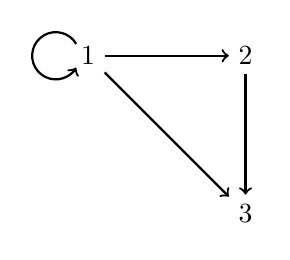
\begin{tikzpicture}
	\node (atom1) at (0,2) {1};
	\node (atom2) at (2,2) {2};
	\node (atom3) at (2,0) {3};
	\draw[->, thick] (atom1)--(atom2);
	\draw[->, thick] (atom1)--(atom3);
	\draw[->, thick] (atom1)+(-0.15,0.15) arc (-330:-30:.3); 
	\draw[->, thick] (atom2) -- (atom3);
	\end{tikzpicture}
\end{center}
Yfirgrip þessarar túlkunar eru fyrstu þrjár heiltölurnar og $Rxy$ er sönn um \emph{x} og \emph{y} ef og aðeins ef það er ör frá \emph{x} til \emph{y} á myndinni. Hér eru nokkrar setningar sem eru sannar samkvæmt þessari túlkun:
\begin{ebullet}
	\item $\forall x \exists y Ryx$ 
	\item $\exists x \forall y Rxy$ \hfill vitni 1
	\item $\exists x \forall y (Ryx \eiff x = y)$ \hfill vitni 1
	\item $\exists x \exists y \exists z (\enot y = z \eand Rxy \eand Rzx)$ \hfill vitni 2
	\item $\exists x \forall y \enot Rxy$ \hfill vitni 3
	\item $\exists x (\exists y Ryx \eand \enot \exists y Rxy)$ \hfill vitni 3
\end{ebullet}
Þetta sýnir að allar þessar setningar eru rökfræðilega samkvæmar. Við getum notfært okkur það til að búa til fleiri og fleiri \emph{ógildar} rökfærslur. Til dæmis:
\begin{align*}
\forall x \exists y Ryx, \exists x \forall y Rxy  &\therefore  \forall x \exists y Rxy\\
\exists x \forall y Rxy, \exists x \forall y \enot Rxy & \therefore \enot \exists x \exists y \exists z (\enot y = z \eand Rxy \eand Rzx)
\end{align*}
og margar fleiri.
\factoidbox{
	Ef til er túlkun þar sem $\meta{A}_1, \meta{A}_2, \ldots, \meta{A}_n$  eru allar sannar og $\meta{C}$ ósönn, þá er:
	\begin{ebullet}
		\item$\meta{A}_1, \meta{A}_2, \ldots, \meta{A}_n \therefore \meta{C}$ \emph{ógild}; og
	\item $\meta{A}_1, \meta{A}_2, \ldots, \meta{A}_n \nentails \meta{C}$; og
	\item 
	 $\meta{A}_1, \meta{A}_2, \ldots, \meta{A}_n, \enot \meta{C}$ eru rökfræðilega samkvæmar.
\end{ebullet}}
Túlkun sem sýnir að tiltekin setning sé \emph{ekki} röksannindi eða að einhverja setningu leiði ekki af annarri er kölluð \emph{gagntúlkun} eða \emph{gagnlíkan}.

Ég vil að lokum minna á sambandið milli gildis og rökfræðilegrar afleiðingar. Umsagnarökfræðin er umtaksmál og hunsar því alls konar blæbrigði mannlegs máls. Það geta því verið aðrar ástæður fyrir því að rökfærsla er gild en umsagnarökfræðin getur fangað. Hér er dæmi:
\begin{earg}
	\item[] Allir kettir eru dauðlegir
	\item[Þar af leiðir:] Allar læður eru dauðlegar
\end{earg}
Þetta er gild rökfærsla. Allar læður eru kettir, svo það er ómögulegt fyrir forsenduna að vera sanna og niðurstöðuna ósanna. Við gætum reynt að þýða þessa rökfærslu yfir á táknmál umsagnarökfræði svona:
$$\forall x(Kx \eif Dx) \therefore \forall x(Lx \eif  Dx)$$
Það er hins vegar lítið mál að finna gagntúlkun sem sýnir að $\forall x (Kx \eif Dx) \nentails \forall x (Lx \eif Dx)$. (Finnið slíka túlkun.) Það væri því rangt að draga þá ályktun að þessi rökfærsla sé ógild, bara af því að til er gagntúlkun fyrir samsvarandi rökfærslu á máli setningarökfræði. Slík þýðing gengur bara ef ekkert mikilvægt tapast í þýðingunni.

\practiceproblems

\problempart
\label{pr.Contingent}
Sýnið að eftirfarandi setningar séu hvorki röksannindi né mótsagnir:
\begin{earg}
\item  $Da \eand Db$
\item  $\exists x Txh$
\item  $Pm \eand \enot\forall x Px$
\item $\forall z Jz \eiff \exists y Jy$
\item $\forall x (Wxmn \eor \exists yLxy)$
\item $\exists x (Gx \eif \forall y My)$
\item $\exists x (x = h \eand x = i)$
\end{earg}

\problempart
\label{pr.NotEquiv}
Sýnið að eftirfarandi setningapör séu ekki rökfræðilega jafngild.
\begin{earg}
\item $Ja$, $Ka$
\item $\exists x Jx$, $Jm$
\item $\forall x Rxx$, $\exists x Rxx$
\item $\exists x Px \eif Qc$, $\exists x (Px \eif Qc)$
\item $\forall x(Px \eif \enot Qx)$, $\exists x(Px \eand \enot Qx)$
\item $\exists x(Px \eand Qx)$, $\exists x(Px \eif Qx)$
\item $\forall x(Px\eif Qx)$, $\forall x(Px \eand Qx)$
\item $\forall x\exists y Rxy$, $\exists x\forall y Rxy$
\item $\forall x\exists y Rxy$, $\forall x\exists y Ryx$
\end{earg}



\problempart
Sýnið að eftirfarandi setningar séu samkvæmar:
\begin{earg}
\item $Ma, \enot Na, Pa, \enot Qa$
\item $Lee, Leg, \enot Lge, \enot Lgg$
\item $\enot (Ma \eand \exists x Ax), Ma \eor Fa, \forall x(Fx \eif Ax)$
\item $Ma \eor Mb, Ma \eif \forall x \enot Mx$
\item $\forall y Gy, \forall x (Gx \eif Hx), \exists y \enot Iy$
\item $\exists x(Bx \eor Ax), \forall x \enot Cx, \forall x\bigl[(Ax \eand Bx) \eif Cx\bigr]$
\item $\exists x Xx, \exists x Yx, \forall x(Xx \eiff \enot Yx)$
\item $\forall x(Px \eor Qx), \exists x\enot(Qx \eand Px)$
\item $\exists z(Nz \eand Ozz), \forall x\forall y(Oxy \eif Oyx)$
\item $\enot \exists x \forall y Rxy, \forall x \exists y Rxy$
\item $\enot Raa$, $\forall x (x=a \eor Rxa)$
\item $\forall x\forall y\forall z(x=y \eor y=z \eor x=z)$, $\exists x\exists y\ \enot x= y$
\item $\exists x\exists y(Zx \eand Zy \eand x=y)$, $\enot Zd$, $d=e$
\end{earg}

\problempart
Sýnið að eftirfarandi rökfærslur séu ógildar:
\begin{earg}
\item $\forall x(Ax \eif Bx) \therefore \exists x Bx$
\item $\forall x(Rx \eif Dx), \forall x(Rx \eif Fx) \therefore \exists x(Dx \eand Fx)$
\item $\exists x(Px\eif Qx) \therefore \exists x Px$
\item $Na \eand Nb \eand Nc \therefore \forall x Nx$
\item $Rde, \exists x Rxd \therefore Red$
\item $\exists x(Ex \eand Fx), \exists x Fx \eif \exists x Gx \therefore \exists x(Ex \eand Gx)$
\item $\forall x Oxc, \forall x Ocx \therefore \forall x Oxx$
\item $\exists x(Jx \eand Kx), \exists x \enot Kx, \exists x \enot Jx \therefore \exists x(\enot Jx \eand \enot Kx)$
\item $Lab \eif \forall x Lxb, \exists x Lxb \therefore Lbb$
\item $\forall x(Dx \eif \exists y Tyx) \therefore \exists y \exists z\ \enot y= z$
\end{earg}

\chapter{Takmarkanir túlkana og umsagnarökfræðinnar}

\section{Röksannindi og mótsagnir}
Við getum sýnt að setning sé \emph{ekki} röksannindi með því að finna bara eina einustu túlkun sem sýnir að setningin sé ósönn. En ef við viljum á hinn bóginn sýna að setning \emph{sé} röksannindi þá skiptir ekki máli hversu margar túlkanir við finnum þar sem hún er sönn, það er alltaf möguleiki að til sé einhver önnur túlkun þar sem hún er ósönn. Við þyrftum því að geta hugsað upp óendanlega margar túlkanir!

Stundum getum við þó neglt niður tiltölulega auðveldlega hvernig allar túlkanir fyrir tilteknar setningar hljóta að vera. Til dæmis, þá er tiltölulega auðvelt að sýna að $Raa\eiff Raa$ séu röksannindi: 
	\begin{quote}
		\label{allmodels1}
		Túlkun fyrir tiltekna setningu verður að tiltaka merkinga allra nafna sem kemur fyrir í henni. Ef $Raa$ er sönn í tiltekinni túlkun, þá er $Raa \eiff Raa$ sönn í þeirri túlkun. En ef $Raa$ er ósönn í einhverri túlkun, þá er $Raa \eiff Raa$ sönn í þeirri túlkun. Þetta eru einu möguleikarnir. $Raa \eiff Raa$ er því sönn fyrir allar túlkanir. Setningin er því röksannindi.
	\end{quote}
Þetta er gild rökfærsla og niðurstaða hennar er sönn. En þetta er auðvitað ekki rökfærsla \emph{á máli umsagnarökfræði}, heldur á mæltu máli \emph{um} umsagnarökfræði---þetta er rökfærsla á framsetningarmálinu.

Takið líka eftir því að setningin inniheldur enga magnara og við þurfum því ekki að spá neitt sérstaklega í því hvernig túlka beri $a$ eða $R$. Það eina sem skipti máli var að \emph{sama hvernig við túlkum þessi tákn, þá hefði $Raa$ eitthvað sanngildi}. Þessi rökfærsla hefði allt eins getað verið um setningar í setningarökfræði.	

Skoðum annað dæmi. Setningin $\forall x(Rxx\eiff Rxx)$ ætti að sjálfsögðu að vera röksannindi, rétt eins og fyrra dæmi. En það er ekki jafn auðvelt að sýna af hverju. Við getum ekki sagt að $Rxx \eiff Rxx$ sé satt fyrir allar túlkanir, því $Rxx \eiff Rxx$ er ekki einu sinni setning í umsagnarökfræði (\emph{x} er breyta, ekki nafn.) Við verðum því að reyna rökfærslu á borð við þessa:
	\begin{quote}
		Veljum einhverja túlkun af handahófi. Veljum svo eitthvað stak úr yfirgripinu---köllum það bara „S“. Víkkum svo út túlkunina sem við völdum þannig að nafnið $c$ vísi til S. Þá er $Rcc$ annað hvort sönn eða ósönn. Ef $Rcc$ er sönn, þá er $Rcc \eiff Rcc$ sönn. En ef $Rcc$ er ósönn, þá er $Rcc \eiff Rcc$ líka sönn. Svo hvort heldur sem er, þá er $Rcc$ sönn. En þar sem við völdum túlkun og S af handahófi, þá skiptir það engu máli hvernig við víkkum túlkunina sem við völdum út, $Rcc \eiff Rcc$ verður sönn. En þá er $\forall x (Rxx \eiff Rxx)$ sönn samkvæmt túlkuninni sem við völdum og af því að við völdum hana af handahófi, þá er $\forall x (Rxx \eiff Rxx)$ sönn fyrir allar túlkanir og er því röksannindi.
	\end{quote}
Þetta er ansi langdregið. En því miður er ekkert annað sem við getum gert. Ef við viljum sýna að setning séu röksannindi, þá eigum við engra annarra kosta völ en að sýna eitthvað um allar túlkanir og það er enginn hægðarleikur. Þetta gildir að sjálfsögðu líka um ýmis önnur tilfelli. Til dæmis ef við viljum sýna að:
	\begin{ebullet}
		\item setning sé mótsögn; hér þarf að sýna að hún sé ósönn í öllum túlkunum. 
		\item að tvær setningar séu rökfræðilega jafngildar; hér þurfum við að sýna að þær hafi sama sanngildi í öllum túlkunum.
		\item að eitthvað safn setninga sé ósamkvæmt; hér þurfum við að sýna að ekki sé til túlkun þar sem setningarnar eru allar sannar, það er, að sýna að í hverri einustu túlkun sé að minnsta kosti einn setninganna ósönn.
		\item að rökfærsla sé gild; hér þarf að sýna að niðurstaðan sé sönn í öllum túlkunum þar sem forsendurnar eru sannar.
		\item að einhverja setningu leiði af öðrum setningum.
	\end{ebullet}
Það er mikill munur á þessu og því sem við höfum áður kynnst. Sannleikur setninga í setningafræði er skilgreindur með sanngildadreifingum og hver setning hefur einungis endanlegan fjölda af mögulegum sanngildadreifingum. Við getum notað sanntöflur til að fá yfirsýn yfir allar þessar dreifingar og eru þær í raun aðferð til að meta sanngildi allra setninga í setningarökfræði á vélrænan hátt og óbrigðulan hátt. Við getum með öðrum orðum reiknað út sanngildi allra setninga í setningarökfræði. \emph{En það er ekki til nein slík aðferð í tilfelli umsagnarökfræði}.\footnote{Hér þurfum við samt að fara dálítið varlega. Það hefði vel verið mögulegt að slík almenn aðferð hefði verið til, þrátt fyrir að mögulegar túlkanir séu óendanlega margar. Það er ekki eina ástæðan fyrir þessum vanda. Hins vegar sönnuðu Alonso Church og Alan Turing um miðjan fjórða áratug síðustu aldar að slík aðferð er ekki til.} Umsagnarökfræði er, eins og sagt er, óúrskurðanleg (e.\ \emph{undecidable}). Þetta þýðir þó ekki að það séu til sannar setningar sem umsagnarökfræðin getur ekki sannað, bara að það er ekki til nein aðferð til að finna slíka sönnun. Við höfum þó ekki enn kynnt sannanir til sögunnar fyrir umsagnarrökfræðina, en það er efni næsta kafla.